\documentclass[11pt]{article}
\usepackage[letterpaper,margin=0.9in,top=0.85in,bottom=0.85in]{geometry}
\usepackage{amsmath,amssymb}
\usepackage[most]{tcolorbox}
\usepackage{tikz}
\usepackage{pgfplots}
\pgfplotsset{compat=1.18}
\usepackage{enumitem}
\usepackage{multicol}
\usepackage{xcolor}
\usepackage{titlesec}
\usepackage{fancyhdr}
\usepackage{booktabs}
\usepackage{array}
\usepackage{parskip}
\setlength{\parskip}{4pt}

\definecolor{mainblue}{RGB}{20,80,170}
\definecolor{lightblue}{RGB}{218,232,255}
\definecolor{maingreen}{RGB}{15,120,70}
\definecolor{lightgreen}{RGB}{210,245,225}
\definecolor{mainorange}{RGB}{190,70,0}
\definecolor{lightorange}{RGB}{255,238,215}
\definecolor{mainpurple}{RGB}{90,30,160}
\definecolor{lightpurple}{RGB}{240,230,255}

\tcbuselibrary{skins,breakable}
\tcbset{
  exbox/.style={enhanced,colback=lightblue,colframe=mainblue,
    fonttitle=\bfseries\color{white},
    attach boxed title to top left={yshift=-2mm,xshift=6mm},
    boxed title style={colback=mainblue},
    boxrule=1pt,arc=4pt,left=8pt,right=8pt,top=8pt,bottom=6pt},
  keybox/.style={enhanced,colback=lightorange,colframe=mainorange,
    fonttitle=\bfseries\color{white},
    attach boxed title to top left={yshift=-2mm,xshift=6mm},
    boxed title style={colback=mainorange},
    boxrule=1pt,arc=4pt,left=8pt,right=8pt,top=6pt,bottom=6pt},
  ansbox/.style={enhanced jigsaw,colback=lightgreen,colframe=maingreen,
    fonttitle=\bfseries\color{white},
    attach boxed title to top left={yshift=-2mm,xshift=6mm},
    boxed title style={colback=maingreen},
    boxrule=1pt,arc=4pt,left=8pt,right=8pt,top=8pt,bottom=6pt,breakable},
  tablebox/.style={enhanced,colback=lightpurple,colframe=mainpurple,
    fonttitle=\bfseries\color{white},
    attach boxed title to top left={yshift=-2mm,xshift=6mm},
    boxed title style={colback=mainpurple},
    boxrule=1pt,arc=4pt,left=8pt,right=8pt,top=8pt,bottom=6pt},
}

\pagestyle{fancy}\fancyhf{}
\fancyhead[L]{\small\textit{Math Practice Worksheet}\quad{\color{mainorange}\textbf{FangMath}}}
\fancyhead[R]{\small Name:\underline{\hspace{4cm}}\;Date:\underline{\hspace{1.8cm}}}
\fancyfoot[C]{\small\thepage}
\fancyfoot[R]{\scriptsize\color{gray}\textcopyright\ 2026 FangMath. All rights reserved.}
\renewcommand{\headrulewidth}{0.4pt}

\titleformat{\section}{\large\bfseries\color{mainblue}}{}{0em}
  {\colorbox{mainblue}{\color{white}\;\thesection\;}\;\;}[\vspace{-4pt}\rule{\linewidth}{1pt}]

\newcommand{\smallgrid}{%
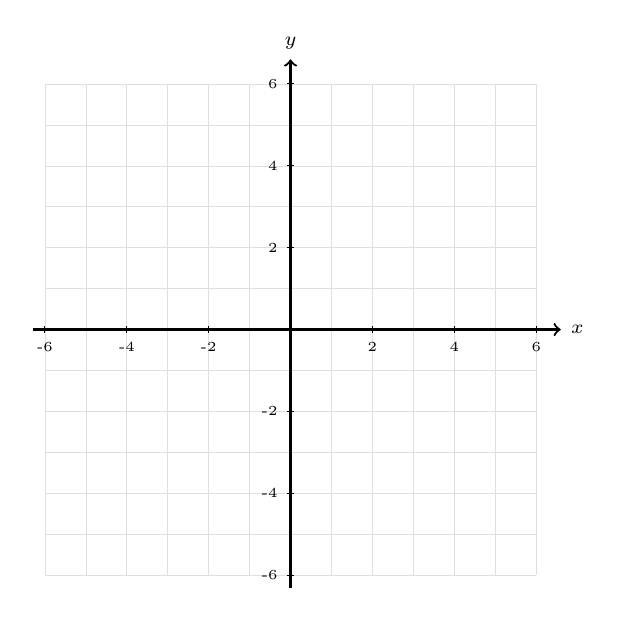
\begin{tikzpicture}[scale=0.52]
  \draw[gray!25,very thin](-6,-6)grid(6,6);
  \draw[->,thick](-6.3,0)--(6.6,0)node[right,font=\scriptsize]{$x$};
  \draw[->,thick](0,-6.3)--(0,6.6)node[above,font=\scriptsize]{$y$};
  \foreach\x in{-6,-4,-2,2,4,6}{\draw(\x,.08)--(\x,-.08)node[below,font=\tiny]{\x};}
  \foreach\y in{-6,-4,-2,2,4,6}{\draw(.08,\y)--(-.08,\y)node[left,font=\tiny]{\y};}
\end{tikzpicture}}

\begin{document}

\begin{center}
{\LARGE\bfseries\color{mainblue}Math Practice Worksheet}\\[4pt]
{\normalsize\color{gray}Pythagorean Theorem $\cdot$ Absolute Value Graphs $\cdot$ Evaluate Functions $\cdot$ Simplify Roots}\\[3pt]
{\small\color{mainorange}\textbf{FangMath}}
\end{center}
\hrule height 1.5pt\vspace{0.8em}

\section{Pythagorean Theorem}

\begin{tcolorbox}[keybox,title={Key Formula}]
In a right triangle with legs $a$, $b$ and hypotenuse $c$ (longest side):\quad
$\boldsymbol{a^2+b^2=c^2}$

\textbf{Find missing side:} isolate the unknown and take the square root.\\
\textbf{Check right triangle:} substitute all three sides --- if $a^2+b^2=c^2$ then \textbf{Yes}, otherwise \textbf{No}.
\end{tcolorbox}

\begin{tcolorbox}[exbox,title={Example}]
\textbf{(a) Find hypotenuse:} $a=3,\,b=4$\qquad
$c^2=3^2+4^2=9+16=25\;\Rightarrow\;c=\sqrt{25}=\boxed{5}$\\[5pt]
\textbf{(b) Find missing leg:} $a=5,\,c=13$\qquad
$b^2=13^2-5^2=169-25=144\;\Rightarrow\;b=\sqrt{144}=\boxed{12}$\\[5pt]
\textbf{(c) Check $(3,4,5)$:}\quad $3^2+4^2=9+16=25=5^2$\;\checkmark\quad\boxed{\text{Yes, right triangle}}
\end{tcolorbox}

\begin{enumerate}[leftmargin=*,label=\textbf{\arabic*.}]
\item Find the hypotenuse: $a=6,\;b=8$.\vspace{1.7cm}
\item Find the hypotenuse: $a=5,\;b=12$.\vspace{1.7cm}
\item Find the hypotenuse: $a=7,\;b=24$.\vspace{1.7cm}
\item Find the hypotenuse: $a=10,\;b=24$.\vspace{1.7cm}
\item Find the missing leg: $a=9,\;c=15$.\vspace{1.7cm}
\item Find the missing leg: $b=8,\;c=17$.\vspace{1.7cm}
\item Find the missing leg: $a=20,\;c=25$.\vspace{1.7cm}
\item Is $(6,\,8,\,10)$ a right triangle?\vspace{1.4cm}
\item Is $(5,\,7,\,9)$ a right triangle?\vspace{1.4cm}
\item Is $(8,\,15,\,17)$ a right triangle?\vspace{1.4cm}
\end{enumerate}

\newpage
\section{Graphing Absolute Value Functions}

\begin{tcolorbox}[tablebox,title={Transformation Summary Table: $y = a|x-h|+k$}]
\renewcommand{\arraystretch}{1.35}
\begin{tabular}{>{\bfseries}p{3.5cm} p{4.5cm} p{5.5cm}}
\toprule
\textbf{Form} & \textbf{Transformation} & \textbf{Effect on Graph} \\
\midrule
$y=|x|$ & Parent function & V-shape, vertex at $(0,0)$, opens up \\
$y=|x|+k$,\; $k>0$ & Vertical shift \textbf{up} & Vertex moves up $k$ units \\
$y=|x|-k$,\; $k>0$ & Vertical shift \textbf{down} & Vertex moves down $k$ units \\
$y=|x-h|$,\; $h>0$ & Horizontal shift \textbf{right} & Vertex moves right $h$ units \\
$y=|x+h|$,\; $h>0$ & Horizontal shift \textbf{left} & Vertex moves left $h$ units \\
$y=a|x|$,\; $a>1$ & Vertical \textbf{stretch} & V becomes \textbf{narrower} \\
$y=a|x|$,\; $0<a<1$ & Vertical \textbf{compression} & V becomes \textbf{wider} \\
$y=-|x|$ & \textbf{Reflection} over $x$-axis & Opens \textbf{downward} \\
$y=a|x-h|+k$ & \textbf{Combined} transformation & Vertex $(h,k)$; up if $a>0$, down if $a<0$ \\
\bottomrule
\end{tabular}
\end{tcolorbox}

\begin{tcolorbox}[keybox,title={Key Concepts}]
\textbf{Vertex} $= (h,\,k)$\quad
$a>0$: opens \textbf{up}\quad
$a<0$: opens \textbf{down}\quad
$|a|>1$: \textbf{narrower}\quad
$0<|a|<1$: \textbf{wider}
\end{tcolorbox}

\begin{tcolorbox}[exbox,title={Example: Graph $y=|x-2|+1$}]
Vertex $(2,1)$; $a=1>0$ opens up; slopes $\pm1$ from vertex.
\hfill
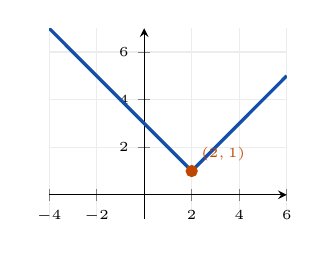
\begin{tikzpicture}
\begin{axis}[width=4.6cm,height=4cm,xmin=-4,xmax=6,ymin=-1,ymax=7,
  axis lines=center,grid=both,grid style={gray!15},
  tick label style={font=\tiny},xtick={-4,-2,...,6},ytick={0,2,...,6}]
\addplot[mainblue,very thick,domain=-4:6,samples=80]{abs(x-2)+1};
\addplot[mainorange,mark=*,mark size=2pt]coordinates{(2,1)};
\node[font=\tiny,mainorange,above right] at (axis cs:2,1) {$(2,1)$};
\end{axis}
\end{tikzpicture}
\end{tcolorbox}

\noindent\textit{Graph each function. Label the vertex and state the transformation(s).}
\medskip

\noindent
\begin{tabular}{@{}p{0.47\linewidth}@{\hspace{0.06\linewidth}}p{0.47\linewidth}@{}}
\textbf{1.}\;$y=|x|$ & \textbf{2.}\;$y=|x|+3$ \\
Vertex:\underline{\hspace{1.5cm}} Trans:\underline{\hspace{2.5cm}} &
Vertex:\underline{\hspace{1.5cm}} Trans:\underline{\hspace{2.5cm}} \\
\smallgrid & \smallgrid \\[4pt]
\textbf{3.}\;$y=|x|-4$ & \textbf{4.}\;$y=|x-3|$ \\
Vertex:\underline{\hspace{1.5cm}} Trans:\underline{\hspace{2.5cm}} &
Vertex:\underline{\hspace{1.5cm}} Trans:\underline{\hspace{2.5cm}} \\
\smallgrid & \smallgrid \\[4pt]
\textbf{5.}\;$y=|x+2|$ & \textbf{6.}\;$y=|x-1|+2$ \\
Vertex:\underline{\hspace{1.5cm}} Trans:\underline{\hspace{2.5cm}} &
Vertex:\underline{\hspace{1.5cm}} Trans:\underline{\hspace{2.5cm}} \\
\smallgrid & \smallgrid \\[4pt]
\textbf{7.}\;$y=|x+3|-2$ & \textbf{8.}\;$y=2|x|$ \\
Vertex:\underline{\hspace{1.5cm}} Trans:\underline{\hspace{2.5cm}} &
Vertex:\underline{\hspace{1.5cm}} Trans:\underline{\hspace{2.5cm}} \\
\smallgrid & \smallgrid \\[4pt]
\textbf{9.}\;$y=-|x|$ & \textbf{10.}\;$y=-|x+2|+4$ \\
Vertex:\underline{\hspace{1.5cm}} Trans:\underline{\hspace{2.5cm}} &
Vertex:\underline{\hspace{1.5cm}} Trans:\underline{\hspace{2.5cm}} \\
\smallgrid & \smallgrid
\end{tabular}

\newpage
\section{Evaluate Functions}

\begin{tcolorbox}[keybox,title={Key Concept}]
To evaluate $f(a)$: replace every $x$ with $a$, then simplify carefully (watch signs!).
\end{tcolorbox}

\begin{tcolorbox}[exbox,title={Example}]
Let $f(x)=3x^2-2x+1$. Find $f(-2)$.\\[4pt]
$f(-2)=3\underbrace{(-2)^2}_{=4}-2(-2)+1=12+4+1=\boxed{17}$
\end{tcolorbox}

\begin{enumerate}[leftmargin=*,label=\textbf{\arabic*.}]
\item $f(x)=2x+5$.\quad Find $f(4)$.\vspace{1.8cm}
\item $g(x)=x^2-3$.\quad Find $g(-2)$.\vspace{1.8cm}
\item $h(x)=3x^2-x+2$.\quad Find $h(3)$.\vspace{1.8cm}
\item $f(x)=|x-5|$.\quad Find $f(1)$.\vspace{1.8cm}
\item $g(x)=\sqrt{x+7}$.\quad Find $g(9)$.\vspace{1.8cm}
\item $f(x)=2x^3-4$.\quad Find $f(-1)$.\vspace{1.8cm}
\item $h(x)=\dfrac{x+3}{x-1}$.\quad Find $h(5)$.\vspace{2.0cm}
\item $f(x)=5x-x^2$.\quad Find $f(-3)$.\vspace{1.8cm}
\item $g(x)=x^2+4x-7$.\quad Find $g(-4)$.\vspace{1.8cm}
\item $h(x)=2|x+1|-3$.\quad Find $h(-5)$.\vspace{1.8cm}
\end{enumerate}

\newpage
\section{Simplify Radical Expressions \textnormal{\small(Hard Level)}}

\begin{tcolorbox}[keybox,title={Key Rules}]
$\sqrt{a^n}=a^{n/2}$\quad
$\sqrt[3]{a^n}=a^{n/3}$\quad
$\sqrt{ab}=\sqrt{a}\cdot\sqrt{b}$\quad
$\sqrt[3]{ab}=\sqrt[3]{a}\cdot\sqrt[3]{b}$\\[4pt]
\textbf{Add/Subtract like radicals only:}\;
$m\sqrt{a}\pm n\sqrt{a}=(m\pm n)\sqrt{a}$\quad
$m\sqrt[3]{a}\pm n\sqrt[3]{a}=(m\pm n)\sqrt[3]{a}$
\end{tcolorbox}

\begin{tcolorbox}[exbox,title={Examples}]
\textbf{(a)}\;$3\sqrt{12}+2\sqrt{27}=6\sqrt{3}+6\sqrt{3}=\boxed{12\sqrt{3}}$\qquad
\textbf{(b)}\;$\sqrt{50}-\sqrt{8}=5\sqrt{2}-2\sqrt{2}=\boxed{3\sqrt{2}}$\\[5pt]
\textbf{(c)}\;$2\sqrt[3]{16}+\sqrt[3]{54}=4\sqrt[3]{2}+3\sqrt[3]{2}=\boxed{7\sqrt[3]{2}}$\qquad
\textbf{(d)}\;$\sqrt{\dfrac{a^8b^6}{a^2b^2}}=\sqrt{a^6b^4}=\boxed{a^3b^2}$
\end{tcolorbox}

\begin{enumerate}[leftmargin=*,label=\textbf{\arabic*.}]
\item $5\sqrt{12}+3\sqrt{75}$\vspace{2cm}
\item $\sqrt{98}-2\sqrt{50}+\sqrt{32}$\vspace{2cm}
\item $3\sqrt[3]{16}+2\sqrt[3]{54}$\vspace{2cm}
\item $4\sqrt[3]{81}-2\sqrt[3]{24}$\vspace{2cm}
\item $\sqrt{48x^5}$\vspace{2cm}
\item $\sqrt[3]{x^{12}y^9}$\vspace{2cm}
\item $\sqrt{\dfrac{a^8b^6}{a^2b^2}}$\vspace{2.2cm}
\item $2\sqrt{45x^5}-x^2\sqrt{20x}$\vspace{2cm}
\item $3\sqrt{8x^3}-x\sqrt{18x}$\vspace{2cm}
\item $\sqrt[3]{24a^6b^3}$\vspace{2cm}
\end{enumerate}

\newpage
\section{Extra Challenge: Simplify Radicals \textnormal{\small(Advanced)}}

\begin{tcolorbox}[keybox,title={Strategies}]
Factor perfect squares/cubes from numbers and variables first, then combine like radicals.\\
$\sqrt[3]{A}\cdot\sqrt[3]{B}=\sqrt[3]{AB}$\qquad
$\dfrac{\sqrt{A}}{\sqrt{B}}=\sqrt{\dfrac{A}{B}}$
\end{tcolorbox}

\begin{enumerate}[leftmargin=*,label=\textbf{\arabic*.}]
\item $5\sqrt{18x^3}+2x\sqrt{50x}-\sqrt{2x^3}$\vspace{2.3cm}
\item $\sqrt[3]{54x^4y^7}$\vspace{2.3cm}
\item $2\sqrt[3]{40}-3\sqrt[3]{135}$\vspace{2.3cm}
\item $\sqrt[3]{16a^7b^4}+2ab\sqrt[3]{2a^4b}$\vspace{2.3cm}
\item $\dfrac{\sqrt{72a^5b^3}}{\sqrt{2ab}}$\vspace{2.5cm}
\item $\sqrt[3]{\dfrac{x^9y^3}{8z^6}}$\vspace{2.5cm}
\item $4\sqrt{75x^3}-x\sqrt{48x}+\sqrt{27x^3}$\vspace{2.3cm}
\item $\sqrt[3]{x^5y^4}\cdot\sqrt[3]{x^4y^2}$\vspace{2.3cm}
\item $3\sqrt{a^3b^5}-ab\sqrt{ab^3}$\vspace{2.3cm}
\item $\sqrt[3]{250}-\sqrt[3]{2}+\sqrt[3]{16}$\vspace{2.3cm}
\end{enumerate}

\newpage
\begin{center}
{\LARGE\bfseries\color{maingreen}--- Answer Key ---}
\end{center}
\hrule height 1.5pt\vspace{0.8em}

\begin{tcolorbox}[ansbox,title={Part 1 --- Pythagorean Theorem}]
\begin{enumerate}[leftmargin=*,label=\textbf{\arabic*.},itemsep=3pt]
\item $c^2=36+64=100\;\Rightarrow\;c=\mathbf{10}$
\item $c^2=25+144=169\;\Rightarrow\;c=\mathbf{13}$
\item $c^2=49+576=625\;\Rightarrow\;c=\mathbf{25}$
\item $c^2=100+576=676\;\Rightarrow\;c=\mathbf{26}$
\item $b^2=225-81=144\;\Rightarrow\;b=\mathbf{12}$
\item $a^2=289-64=225\;\Rightarrow\;a=\mathbf{15}$
\item $b^2=625-400=225\;\Rightarrow\;b=\mathbf{15}$
\item $36+64=100=10^2$\;\checkmark\;\textbf{Yes}
\item $25+49=74\neq 81$\;\textbf{No}
\item $64+225=289=17^2$\;\checkmark\;\textbf{Yes}
\end{enumerate}
\end{tcolorbox}

\vspace{0.5em}

\begin{tcolorbox}[ansbox,title={Part 2 --- Graphing Absolute Value}]
\begin{multicols}{2}
\begin{enumerate}[leftmargin=*,label=\textbf{\arabic*.},itemsep=2pt]
\item Vertex $(0,0)$; parent
\item Vertex $(0,3)$; up 3
\item Vertex $(0,-4)$; down 4
\item Vertex $(3,0)$; right 3
\item Vertex $(-2,0)$; left 2
\item Vertex $(1,2)$; right 1, up 2
\item Vertex $(-3,-2)$; left 3, down 2
\item Vertex $(0,0)$; narrower
\item Vertex $(0,0)$; opens down
\item Vertex $(-2,4)$; left 2, up 4, opens down
\end{enumerate}
\end{multicols}
\medskip
\noindent
\begin{tabular}{@{}llll@{}}
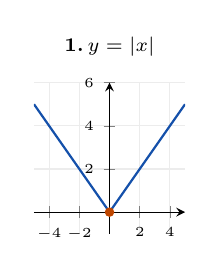
\begin{tikzpicture}
\begin{axis}[title={\scriptsize\textbf{1.}\,$y=|x|$},width=3.5cm,height=3.5cm,
  xmin=-5,xmax=5,ymin=-1,ymax=6,axis lines=center,grid=both,grid style={gray!15},
  tick label style={font=\tiny},xtick={-4,-2,...,4},ytick={0,2,...,6}]
\addplot[mainblue,thick,domain=-5:5]{abs(x)};
\addplot[mainorange,mark=*,mark size=1.5pt]coordinates{(0,0)};
\end{axis}\end{tikzpicture}
&
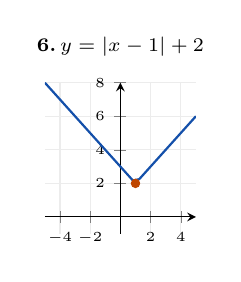
\begin{tikzpicture}
\begin{axis}[title={\scriptsize\textbf{6.}\,$y=|x-1|+2$},width=3.5cm,height=3.5cm,
  xmin=-5,xmax=5,ymin=-1,ymax=8,axis lines=center,grid=both,grid style={gray!15},
  tick label style={font=\tiny},xtick={-4,-2,...,4},ytick={0,2,...,8}]
\addplot[mainblue,thick,domain=-5:5]{abs(x-1)+2};
\addplot[mainorange,mark=*,mark size=1.5pt]coordinates{(1,2)};
\end{axis}\end{tikzpicture}
&
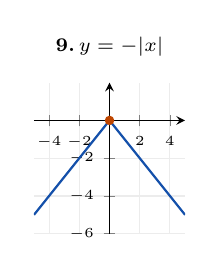
\begin{tikzpicture}
\begin{axis}[title={\scriptsize\textbf{9.}\,$y=-|x|$},width=3.5cm,height=3.5cm,
  xmin=-5,xmax=5,ymin=-6,ymax=2,axis lines=center,grid=both,grid style={gray!15},
  tick label style={font=\tiny},xtick={-4,-2,...,4},ytick={-6,-4,...,0}]
\addplot[mainblue,thick,domain=-5:5]{-abs(x)};
\addplot[mainorange,mark=*,mark size=1.5pt]coordinates{(0,0)};
\end{axis}\end{tikzpicture}
&
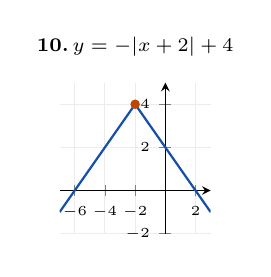
\begin{tikzpicture}
\begin{axis}[title={\scriptsize\textbf{10.}\,$y=-|x+2|+4$},width=3.5cm,height=3.5cm,
  xmin=-7,xmax=3,ymin=-2,ymax=5,axis lines=center,grid=both,grid style={gray!15},
  tick label style={font=\tiny},xtick={-6,-4,...,2},ytick={-2,0,...,4}]
\addplot[mainblue,thick,domain=-7:3]{-abs(x+2)+4};
\addplot[mainorange,mark=*,mark size=1.5pt]coordinates{(-2,4)};
\end{axis}\end{tikzpicture}
\end{tabular}
\end{tcolorbox}

\vspace{0.5em}

\begin{tcolorbox}[ansbox,title={Part 3 --- Evaluate Functions}]
\begin{enumerate}[leftmargin=*,label=\textbf{\arabic*.},itemsep=4pt]
\item $f(4)=8+5=\mathbf{13}$
\item $g(-2)=4-3=\mathbf{1}$
\item $h(3)=27-3+2=\mathbf{26}$
\item $f(1)=|1-5|=\mathbf{4}$
\item $g(9)=\sqrt{16}=\mathbf{4}$
\item $f(-1)=-2-4=\mathbf{-6}$
\item $h(5)=8/4=\mathbf{2}$
\item $f(-3)=-15-9=\mathbf{-24}$
\item $g(-4)=16-16-7=\mathbf{-7}$
\item $h(-5)=2(4)-3=\mathbf{5}$
\end{enumerate}
\end{tcolorbox}

\newpage

\begin{tcolorbox}[ansbox,title={Part 4 --- Simplify Radicals (1--5)}]
\begin{enumerate}[leftmargin=*,label=\textbf{\arabic*.},itemsep=7pt]
\item $5\sqrt{12}+3\sqrt{75}=10\sqrt{3}+15\sqrt{3}=\boldsymbol{25\sqrt{3}}$
\item $\sqrt{98}-2\sqrt{50}+\sqrt{32}=7\sqrt{2}-10\sqrt{2}+4\sqrt{2}=\boldsymbol{\sqrt{2}}$
\item $3\sqrt[3]{16}+2\sqrt[3]{54}=6\sqrt[3]{2}+6\sqrt[3]{2}=\boldsymbol{12\sqrt[3]{2}}$
\item $4\sqrt[3]{81}-2\sqrt[3]{24}=12\sqrt[3]{3}-4\sqrt[3]{3}=\boldsymbol{8\sqrt[3]{3}}$
\item $\sqrt{48x^5}=\sqrt{16\cdot3\cdot x^4\cdot x}=\boldsymbol{4x^2\sqrt{3x}}$
\end{enumerate}
\end{tcolorbox}

\vspace{0.5em}

\begin{tcolorbox}[ansbox,title={Part 4 --- Simplify Radicals (6--10)}]
\begin{enumerate}[leftmargin=*,label=\textbf{\arabic*.},itemsep=7pt,start=6]
\item $\sqrt[3]{x^{12}y^9}=x^{12/3}\cdot y^{9/3}=\boldsymbol{x^4y^3}$
\item $\sqrt{a^6b^4}=\boldsymbol{a^3b^2}$
\item $2\sqrt{45x^5}-x^2\sqrt{20x}=6x^2\sqrt{5x}-2x^2\sqrt{5x}=\boldsymbol{4x^2\sqrt{5x}}$
\item $3\sqrt{8x^3}-x\sqrt{18x}=6x\sqrt{2x}-3x\sqrt{2x}=\boldsymbol{3x\sqrt{2x}}$
\item $\sqrt[3]{24a^6b^3}=\sqrt[3]{8\cdot3\cdot a^6\cdot b^3}=\boldsymbol{2a^2b\sqrt[3]{3}}$
\end{enumerate}
\end{tcolorbox}

\vspace{0.5em}

\begin{tcolorbox}[ansbox,title={Part 5 --- Extra Challenge (1--5)}]
\begin{enumerate}[leftmargin=*,label=\textbf{\arabic*.},itemsep=7pt]
\item $5\sqrt{18x^3}+2x\sqrt{50x}-\sqrt{2x^3}=15x\sqrt{2x}+10x\sqrt{2x}-x\sqrt{2x}=\boldsymbol{24x\sqrt{2x}}$
\item $\sqrt[3]{54x^4y^7}=\sqrt[3]{27\cdot2\cdot x^3\cdot x\cdot y^6\cdot y}=\boldsymbol{3xy^2\sqrt[3]{2xy}}$
\item $2\sqrt[3]{40}-3\sqrt[3]{135}=4\sqrt[3]{5}-9\sqrt[3]{5}=\boldsymbol{-5\sqrt[3]{5}}$
\item $\sqrt[3]{16a^7b^4}+2ab\sqrt[3]{2a^4b}=2a^2b\sqrt[3]{2ab}+2a^2b\sqrt[3]{2ab}=\boldsymbol{4a^2b\sqrt[3]{2ab}}$
\item $\dfrac{\sqrt{72a^5b^3}}{\sqrt{2ab}}=\sqrt{36a^4b^2}=\boldsymbol{6a^2b}$
\end{enumerate}
\end{tcolorbox}

\vspace{0.5em}

\begin{tcolorbox}[ansbox,title={Part 5 --- Extra Challenge (6--10)}]
\begin{enumerate}[leftmargin=*,label=\textbf{\arabic*.},itemsep=7pt,start=6]
\item $\sqrt[3]{\dfrac{x^9y^3}{8z^6}}=\boldsymbol{\dfrac{x^3y}{2z^2}}$
\item $4\sqrt{75x^3}-x\sqrt{48x}+\sqrt{27x^3}=20x\sqrt{3x}-4x\sqrt{3x}+3x\sqrt{3x}=\boldsymbol{19x\sqrt{3x}}$
\item $\sqrt[3]{x^5y^4}\cdot\sqrt[3]{x^4y^2}=\sqrt[3]{x^9y^6}=\boldsymbol{x^3y^2}$
\item $3\sqrt{a^3b^5}-ab\sqrt{ab^3}=3ab^2\sqrt{ab}-ab^2\sqrt{ab}=\boldsymbol{2ab^2\sqrt{ab}}$
\item $\sqrt[3]{250}-\sqrt[3]{2}+\sqrt[3]{16}=5\sqrt[3]{2}-\sqrt[3]{2}+2\sqrt[3]{2}=\boldsymbol{6\sqrt[3]{2}}$
\end{enumerate}
\end{tcolorbox}

\end{document}
